\noindent\textbf{卤代萘:应用广泛的关键化合物}

除了苯之外,萘也是广为人知的芳香烃之一。因此,萘\textbf{1}的化学被广为研究而且许多萘的衍生物已经被合成了出来。其中,它的卤代物是许多转化中的关键。为此,几乎所有的卤代萘在文献中都有出现。对称化合物的\textsuperscript{1}H与\textsuperscript{13}C
NMR谱都很有特点,这就使得研究者排除可能的不对称化合物来分析对称的化合物。下面让我们来考虑四溴代萘\textbf{2}的异构体们。

\begin{figure}[h]
	\centering
	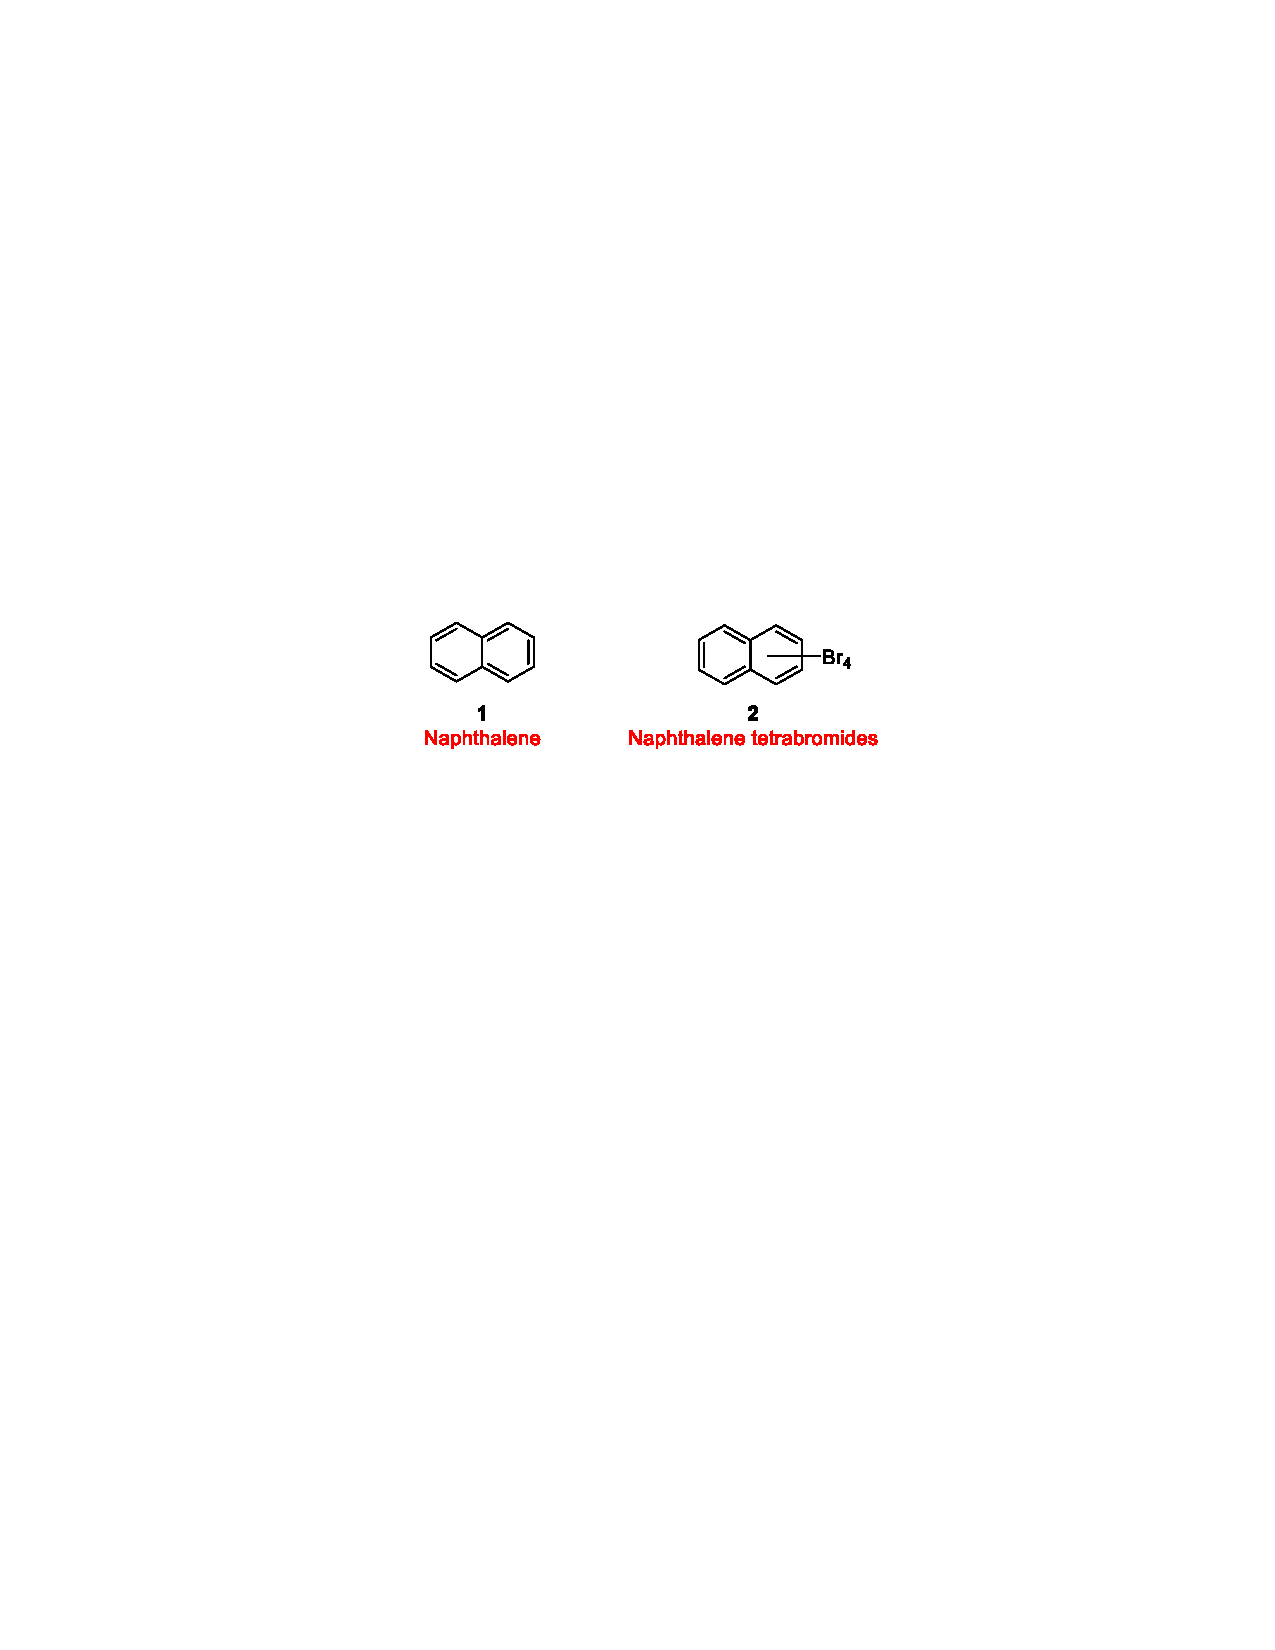
\includegraphics[width=9cm]{./pic/t9-1.pdf}
\end{figure}


\noindent\textbf{9.1.} 画出所有\textsuperscript{13}C
NMR具有三个信号且\textsuperscript{1}H NMR仅含一个信号的四溴代萘异构体。

\noindent\textbf{9.2.} 画出所有\textsuperscript{13}C
NMR具有五个信号的四溴代萘异构体。

\noindent\textbf{9.3.} 画出所有\textsuperscript{13}C
NMR具有六个信号且\textsuperscript{1}H NMR含一个二重峰(\emph{J} = 8-9
Hz)的四溴代萘异构体。

\noindent\textbf{9.4.} 画出所有\textsuperscript{13}C
NMR具有六个信号且\textsuperscript{1}H NMR含一个二重峰(\emph{J} = 1.5-2.0
Hz)的四溴代萘异构体。

\noindent\textbf{动态核磁共振:在NMR中互变异构体的快速转化}

瞬烯\textbf{3}非常容易发生简并的Cope重排。不考虑对映体,瞬烯重排产生的可分辨的互变异构体共有10!/3 = 1,209,600个。这样的重排使得所有的碳原子和氢原子在核磁共振的时间尺度下均是等价的。在足够高的温度下,核磁共振碳谱与氢谱均只显示一个宽峰。然而,在−60 °C,此时Cope重排不可发生,烯基氢跟烷基氢就可以分辨了。

\begin{figure}[h]
	\centering
	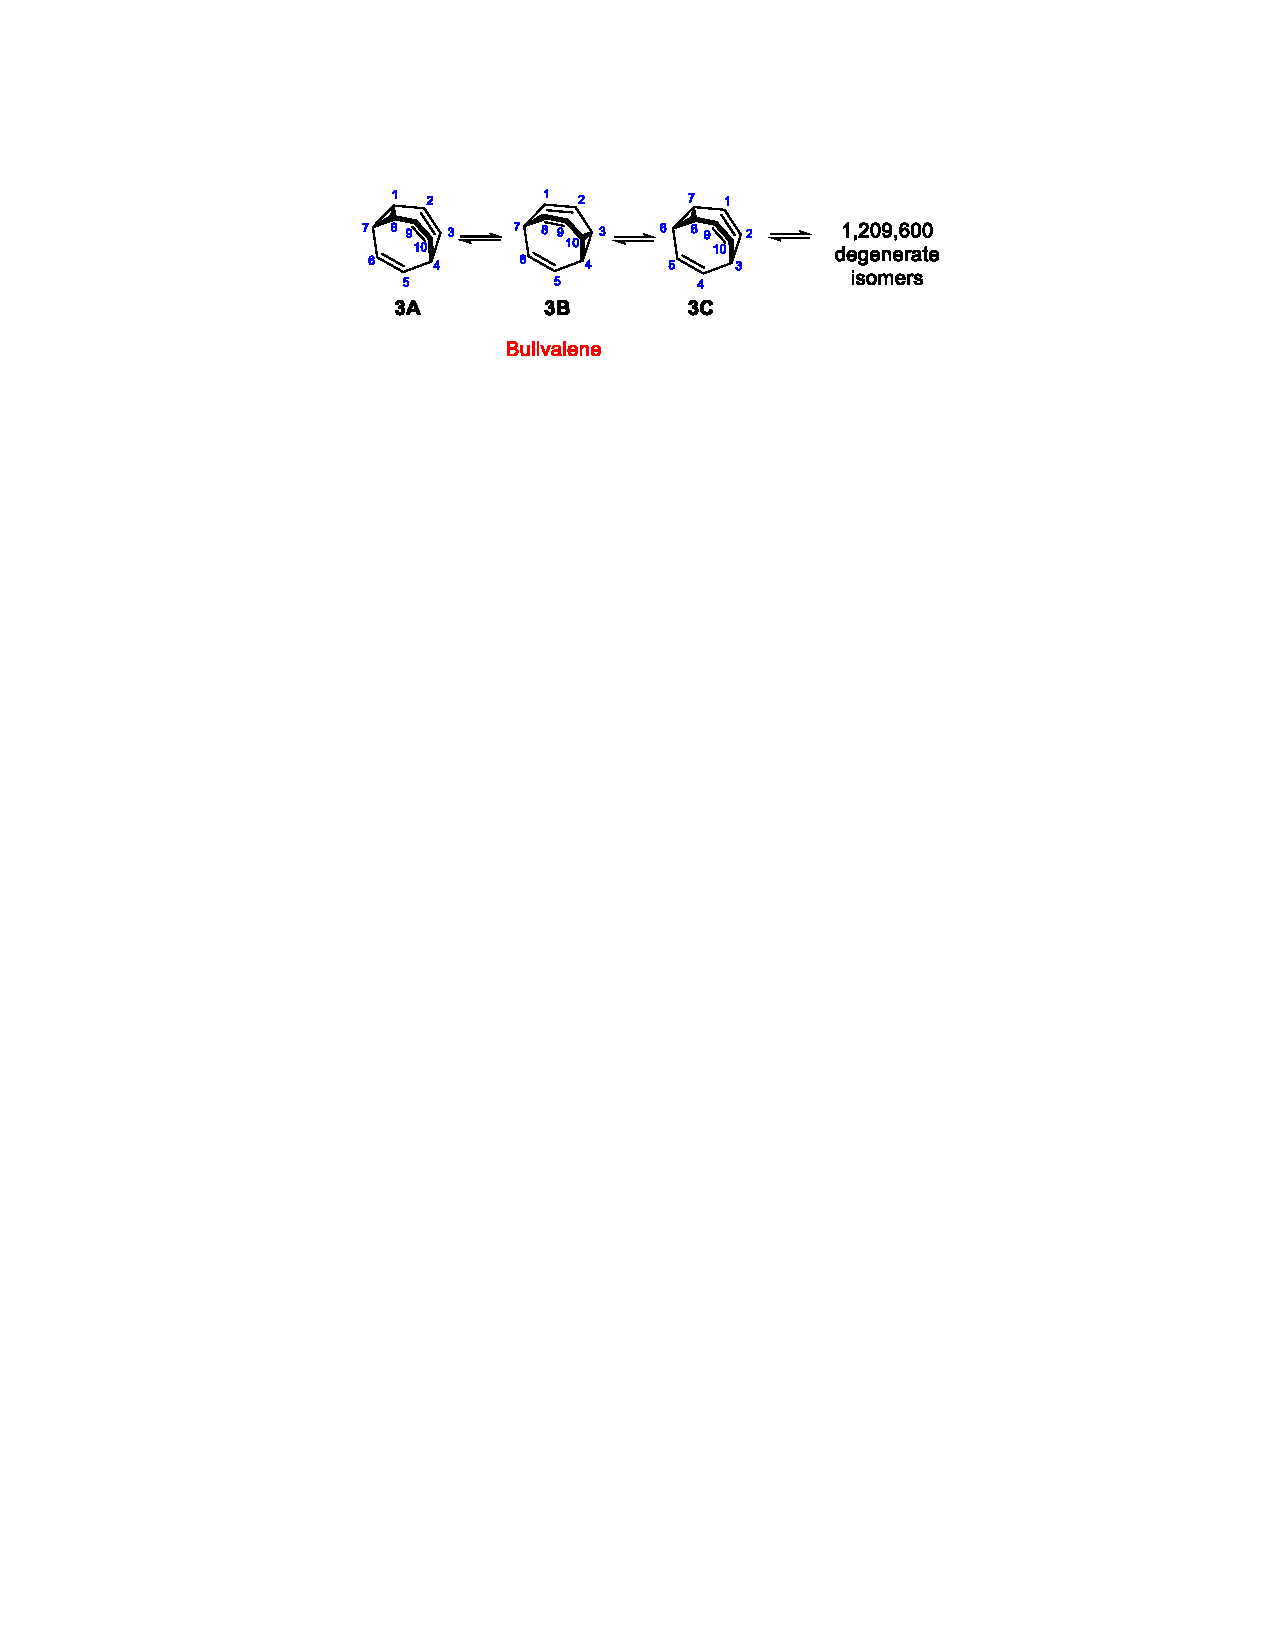
\includegraphics[width=10cm]{./pic/t9-2.pdf}
\end{figure}

\noindent\textbf{9.5.} 低温时,不考虑任何的Cope重排,\textsuperscript{13}C
NMR谱中应有多少个峰?用\textbf{a},\textbf{b},\textbf{c}\ldots{}在分子结构中标记相同的碳原子。

\noindent\textbf{9.6.}
某些分子因互变异构带来的形式上的对称性而给出更清晰的核磁共振谱。根据此信息,您觉得以下化合物的\textsuperscript{13}C
NMR各有多少个峰呢?

\begin{figure}[h]
	\centering
	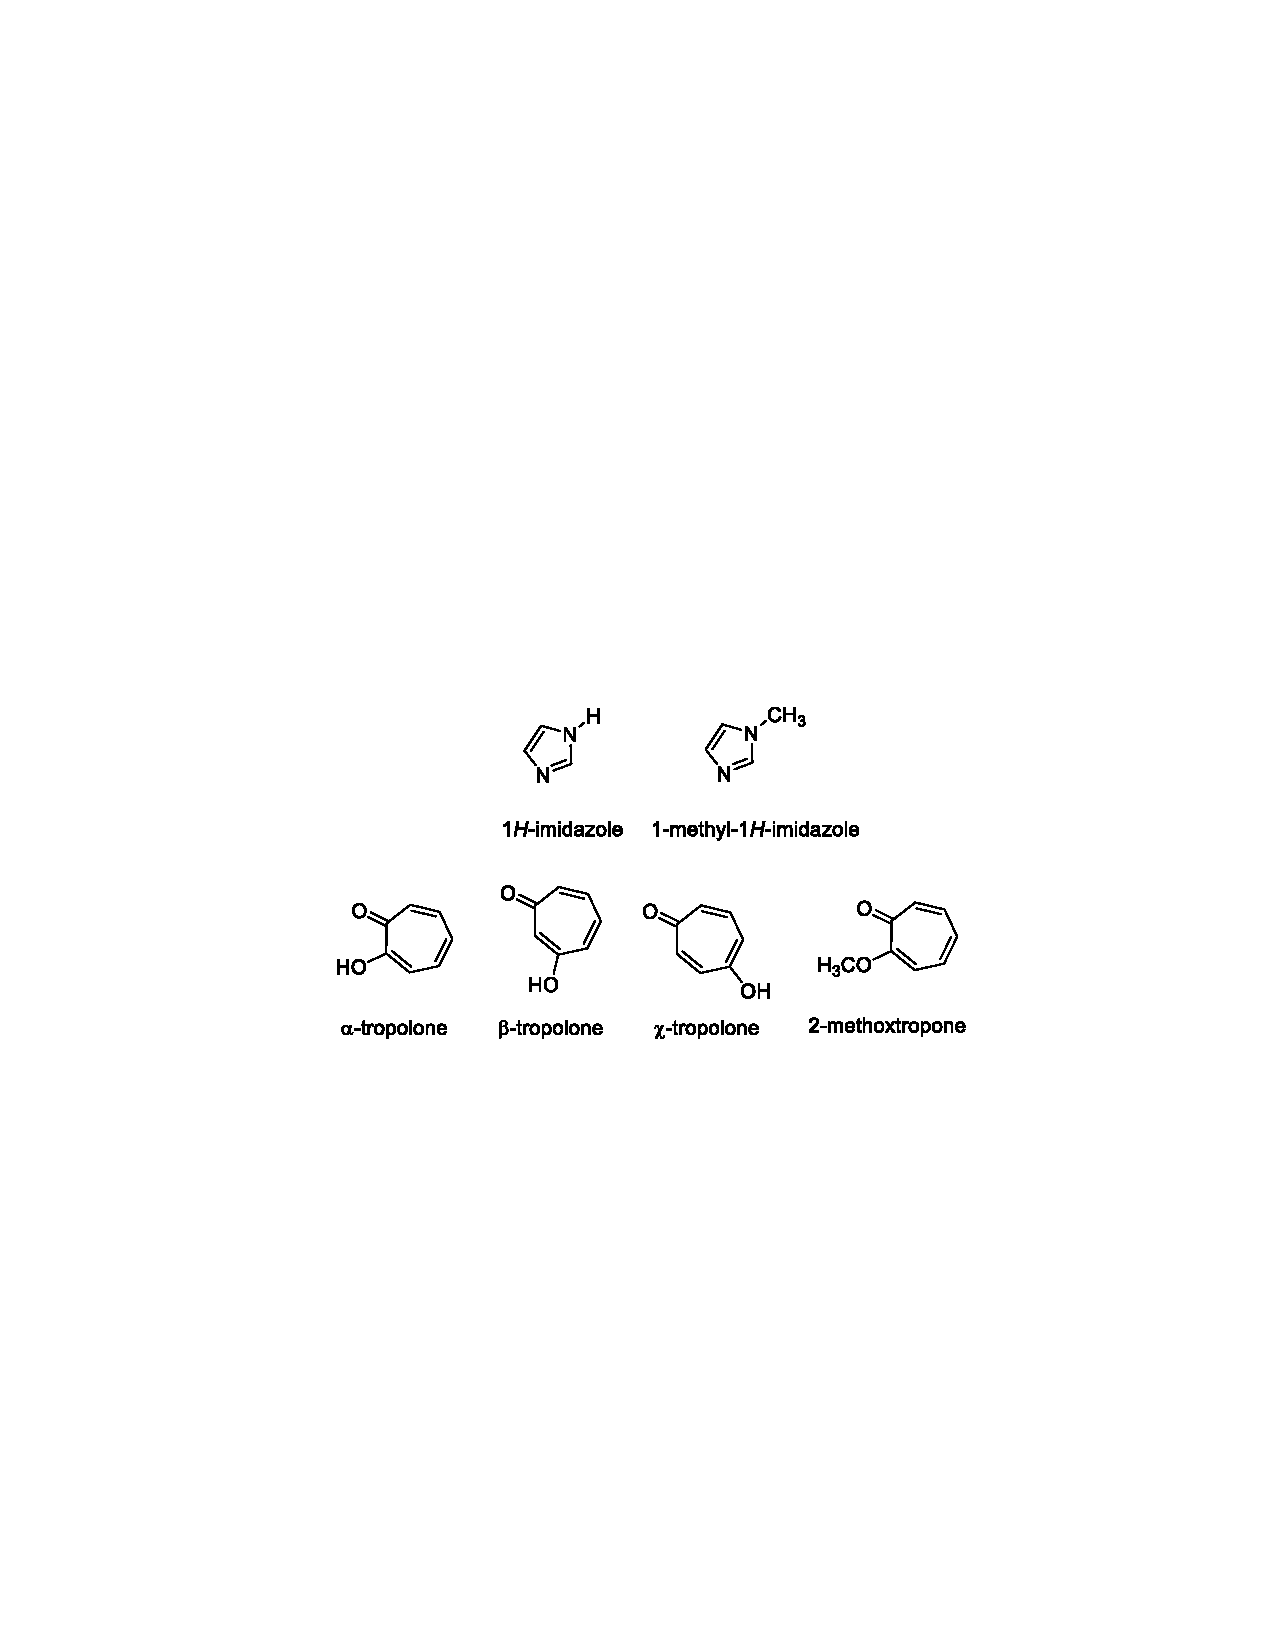
\includegraphics[width=11cm]{./pic/t9-3.pdf}
\end{figure}

\newpage\noindent\textbf{9.7.}
在文献中表明,环庚三烯酚酮衍生物\textbf{4}的\textsuperscript{13}C NMR谱比预料中少了几个峰。

画出合理的共振结构和/或转化来体现这种对称性。您觉得以下化合物的\textsuperscript{13}C NMR各有多少个峰呢?

\begin{figure}[h]
	\centering
	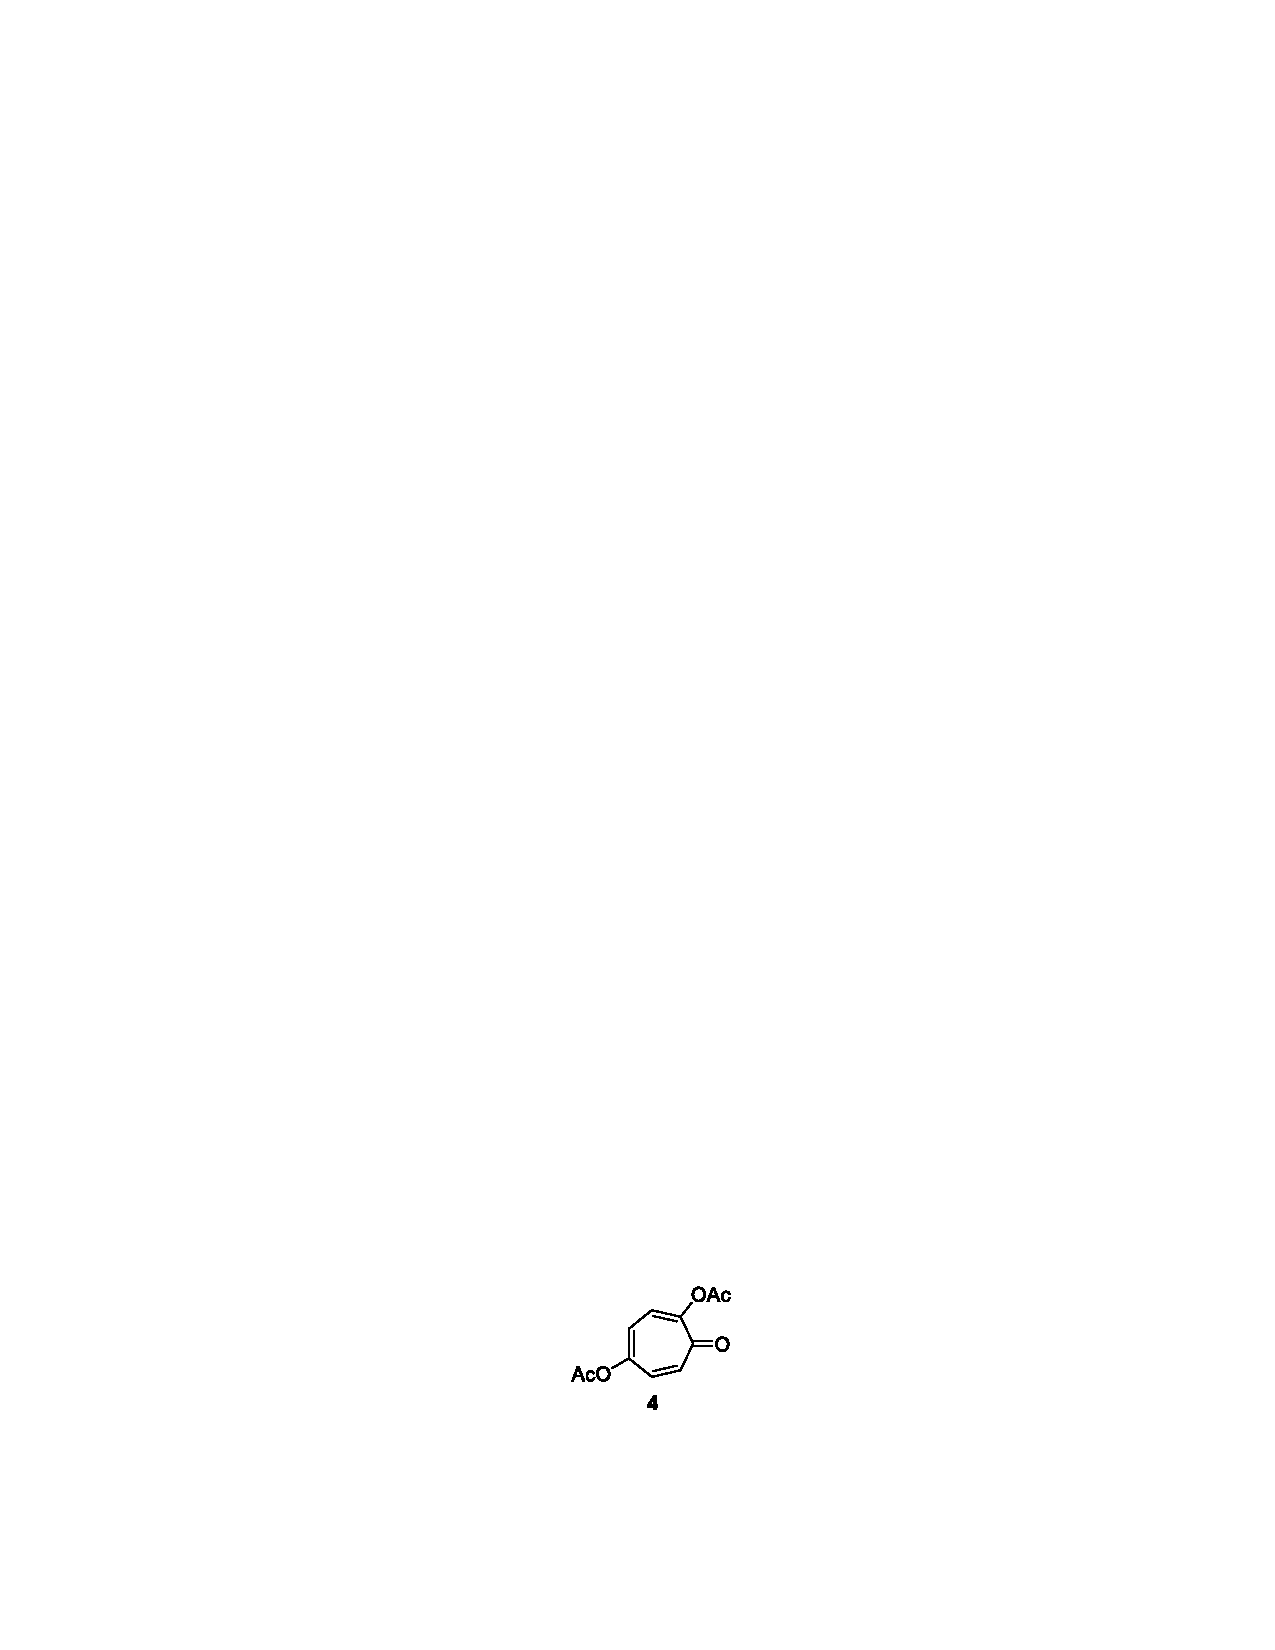
\includegraphics[width=5cm]{./pic/t9-4.pdf}
\end{figure}

\noindent\textbf{双环(桥环)烯烃环氧化的立体化学}

\noindent\textbf{9.8.}考虑以下信息,画出所有在给出的反应条件下可能生成的立体异构体。

\noindent\textbf{提示:A}和\textbf{B}是在\textsuperscript{13}C NMR谱中含有三个峰的异构体,\textbf{C}是在\textsuperscript{13}C NMR谱中含有四个峰的异构体。

\begin{figure}[h]
	\centering
	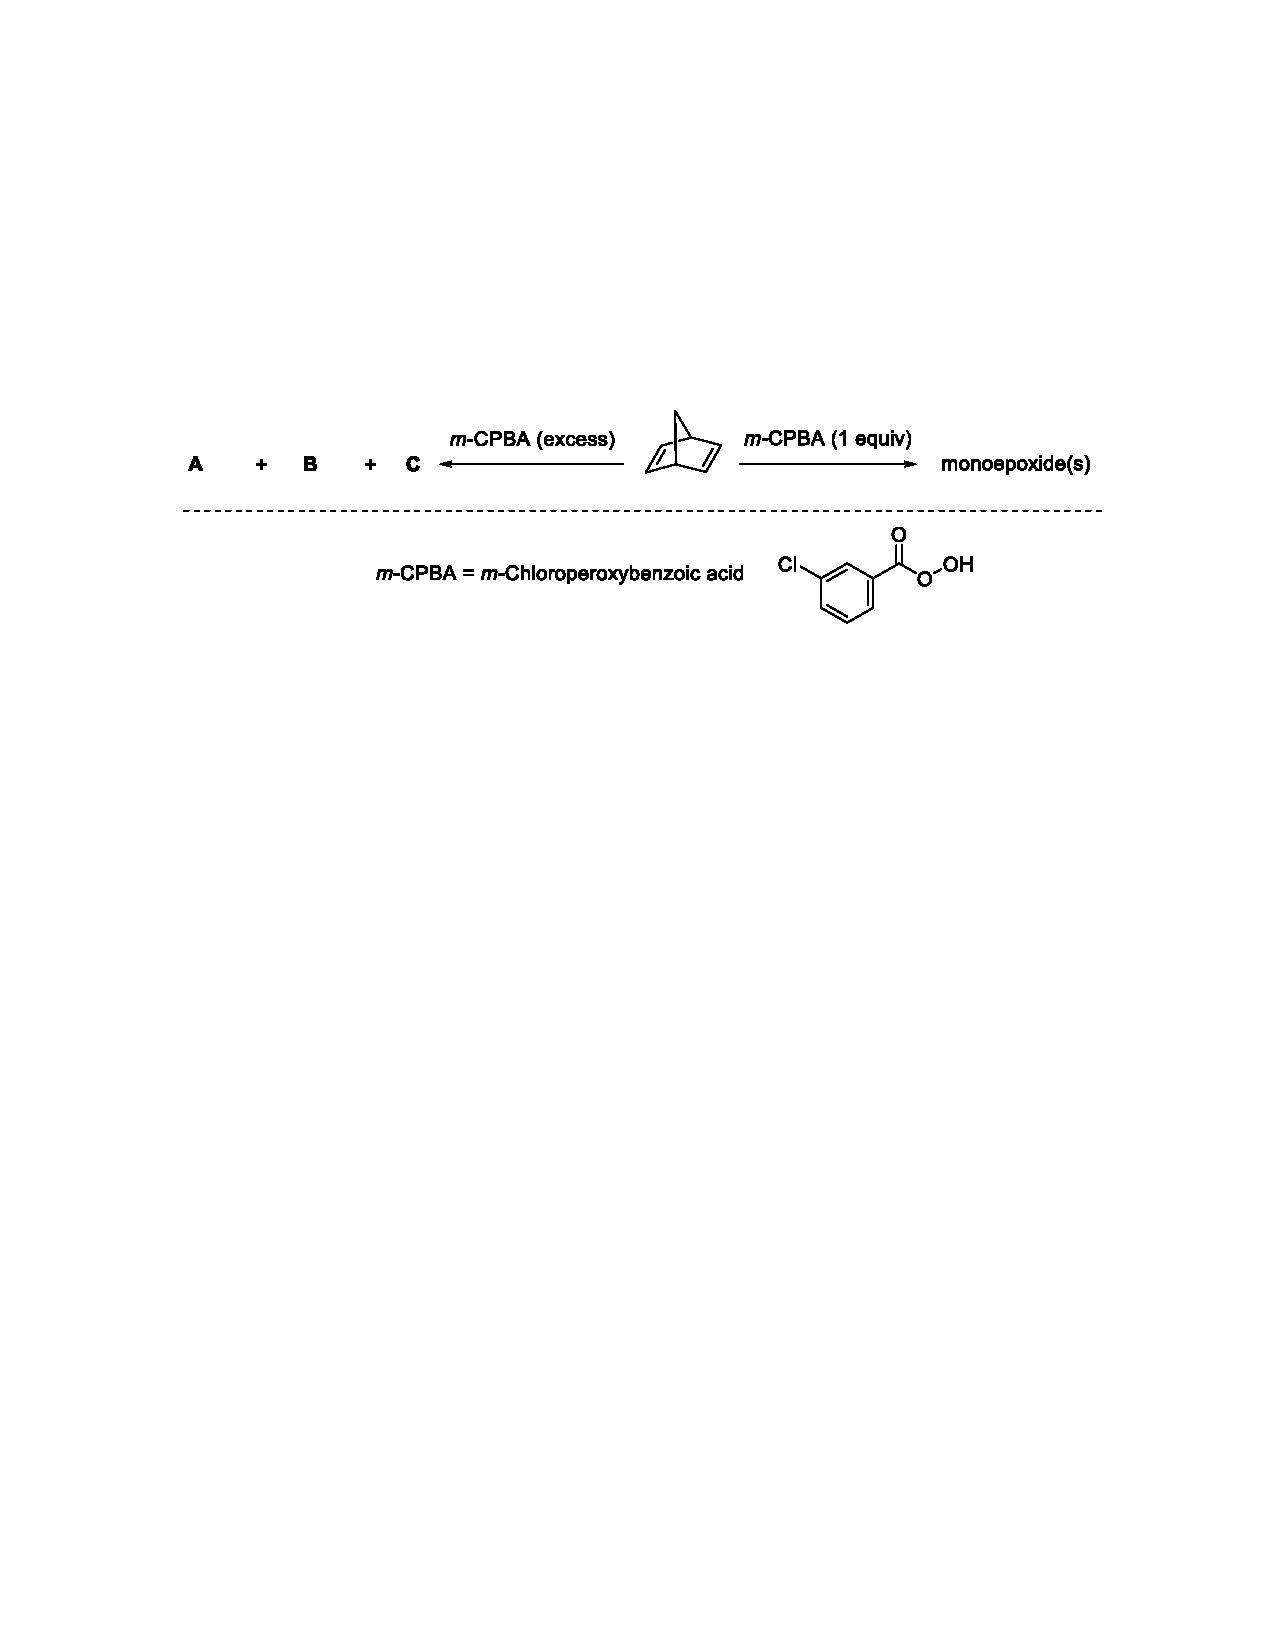
\includegraphics[width=14cm]{./pic/t9-5.pdf}
\end{figure}

\noindent\textbf{9.9.}
画出所有在给出的反应条件下可能生成的立体异构体。您认为在\textsuperscript{13}C
NMR谱中,各产物有多少个峰呢?

\begin{figure}[h!]
	\centering
	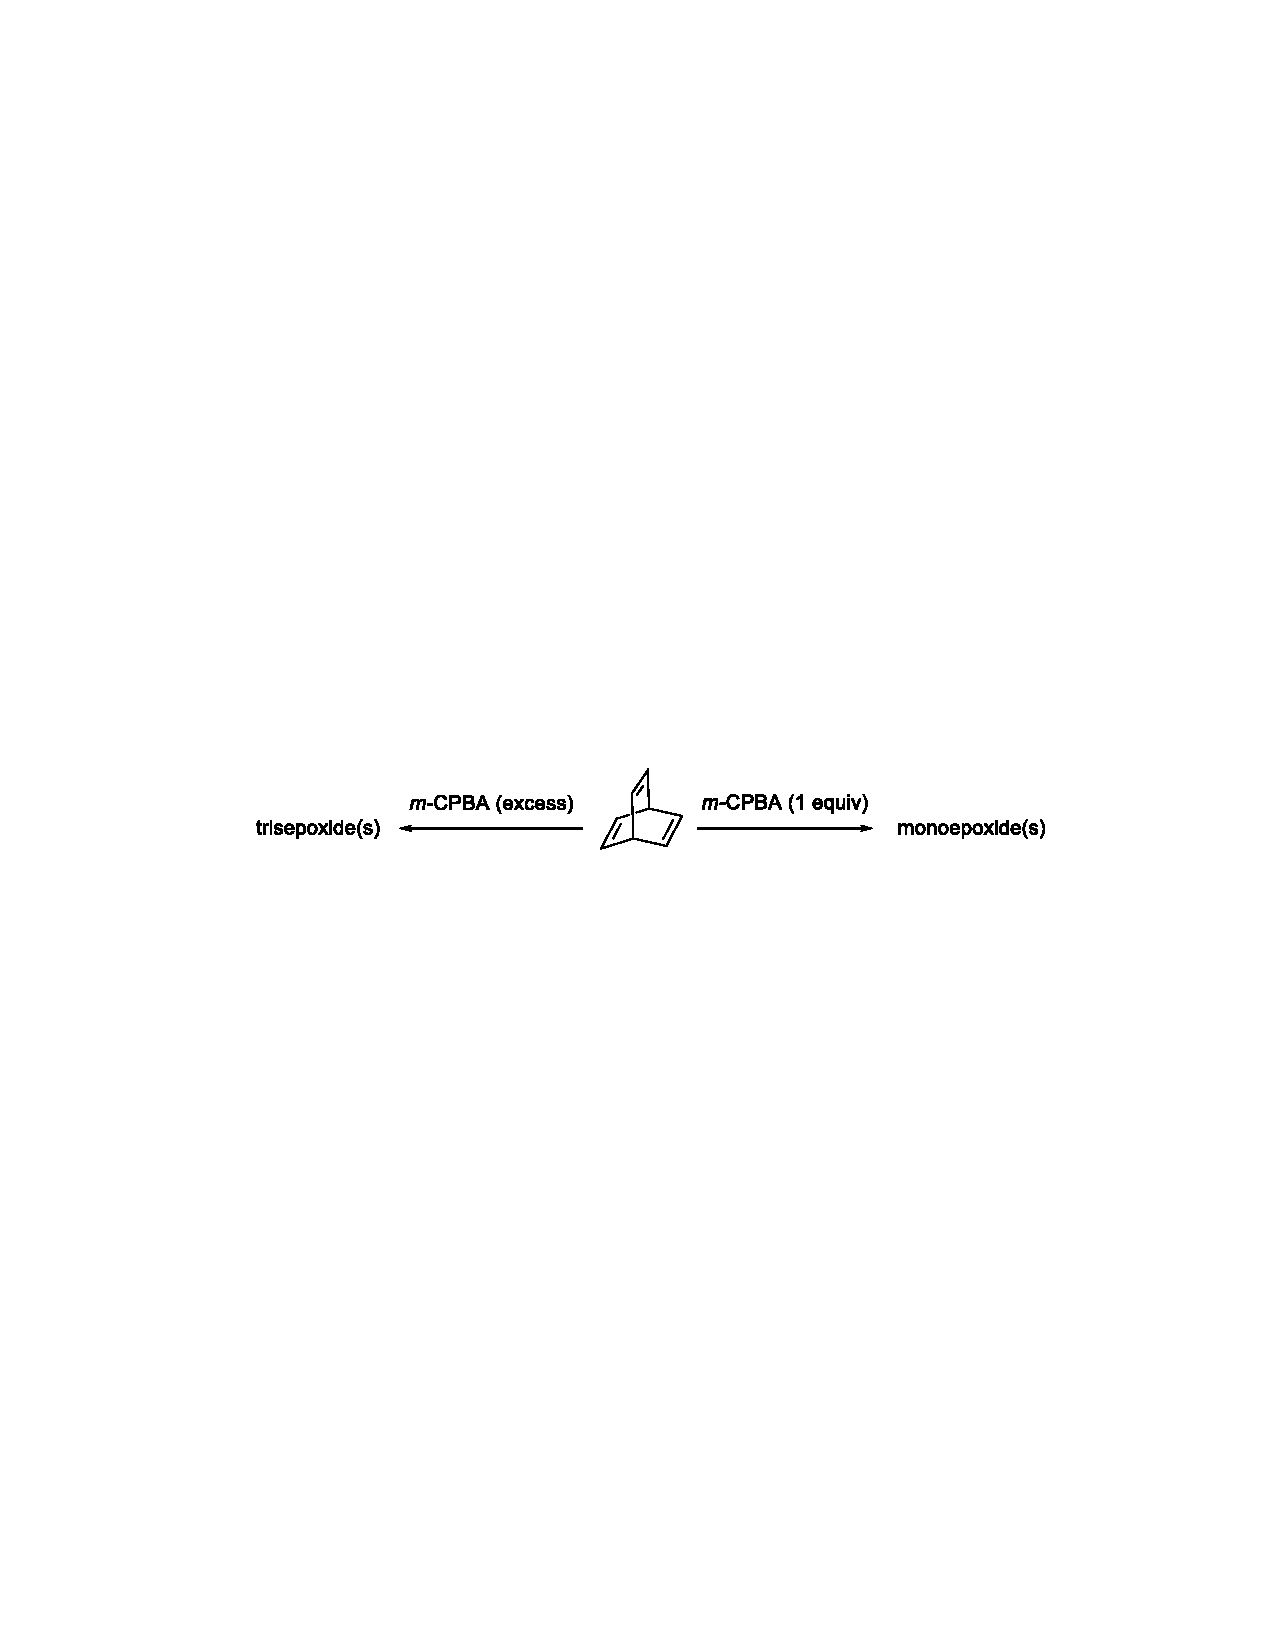
\includegraphics[width=11cm]{./pic/t9-6.pdf}
\end{figure}
